Dado un grafo no dirigido ponderado. Queremos encontrar un subárbol de este grafo que conecte todos los vértices (es decir, es un árbol de expansión) y tiene el menor peso (es decir, la suma de los pesos de todos las aristas es mínima) de todos los árboles de expansión posibles. Este árbol de expansión se denomina árbol de expansión mínimo.

En la imagen de la izquierda puede ver un grafo no dirigido ponderado, y en la imagen de la derecha puede ver el árbol de expansión mínimo correspondiente.

\begin{figure}[h!]
	\centering
	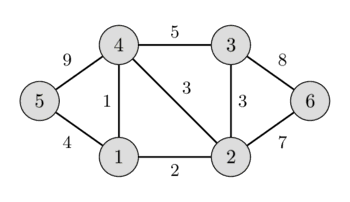
\includegraphics[width=0.45\linewidth]{img/MST_before}
	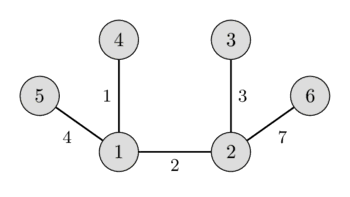
\includegraphics[width=0.45\linewidth]{img/MST_after}
	\label{fig:mstbefore}
\end{figure}
